\addcontentsline{toc}{subsection}{Implicit Differentiation}
\subsection*{Implicit Differentiation}
What we have been doing so far is explicit differentiation, as $y$ has always been an explicit function of $x$. Today, we will continue our journey of taking derivatives but now with equations that are not functions!\\
\begin{tcolorbox}[title= STEPS FOR IMPLICIT DIFFERENTIATION,colframe=black,sharp corners,colback=white,colbacktitle=white,coltitle=black,boxrule=1pt]
    \begin{enumerate}
        \item Differentiate both sides of the equation with respect to $x$, doing $x$ as you normally would. The derivative of $y$ becomes $dy/dx$ or $y'$.
        \item Collect terms with $dy/dx$ on one side of the equation.
        \item Factor out the $dy/dx$.
        \item Solve for $dy/dx$.
    \end{enumerate}
\end{tcolorbox}
\vspace{.15cm}
\noindent\textbf{Examples:} Find $\displaystyle\frac{dy}{dx}$.
\begin{questions}
    \begin{minipage}{.45\linewidth}
    \question $\displaystyle y^2=x$
    \end{minipage}
    \hfill
    \begin{minipage}{.45\linewidth}
    \question $\displaystyle x^2+y^2=25$
    \end{minipage}
    
    \vspace{\stretch{.6}}
    
    \question The Folium of Descartes is $x^3+y^3=9xy$. Find and graph the tangent lines at the points $(4,\,2)$ and $(2,\,4)$.
    
    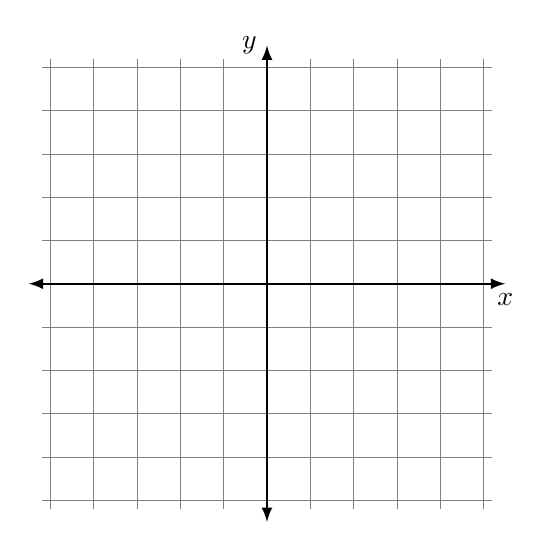
\begin{tikzpicture}[scale=.55]
        \draw[style=help lines] (-5.2,-5.2) grid (5.2,5.2);
        \draw[latex-latex,thick] (-5.5,0) -- (5.5,0) node[below] {$x$};
        \draw[latex-latex,thick] (0,-5.5) -- (0,5.5) node[left] {$y$};
        \draw[thick] plot[raw gnuplot,smooth] function {
            f(x,y) = (x**3)+(y**3)-9*x*y;
            set xrange [-5.2:5.2];
            set yrange [-5.2:5.2];
            set view 0,0;
            set isosample 500,500;
            set cont base;
            set cntrparam levels incre 0,0.1,0;
            unset surface;
            splot f(x,y);
        };
    \end{tikzpicture}
    
    \vspace{\stretch{.1}}
    
    \newpage
    
    \question The line that is normal to the curve $y=x^2+2x-3$ at $(1,\,0)$ intersects the curve at what other point?
    \vspace{\stretch{1}}
    
\end{questions}


\textbf{Example:} Find $\displaystyle\frac{d^2y}{dx^2}$ for $2x^3-3y^2=8$.
\vspace{\stretch{2}}

Second derivatives of Implicit Functions is a skill that is always exercised on the AP Exam. The level of simplification might vary, but the overall procedure and \textit{form} of the final answer is important.

\newpage

Two more examples of second derivatives (time-permitting):
\begin{questions}
    \question $\displaystyle 5y^2+2=5x^2$
    \vspace{\stretch{1}}
    
    \question $y+\cos y=x+1$
    \vspace{\stretch{1}}
\end{questions}

\newpage
